\subsection{Verificar la Correcta Sintaxis de los Archivos de Configuración}

Debido a que la mayoría de los errores encontrados en la configuración de Bacula son resultado de una sintaxis incorrecta, y estos errores suelen impedir que los demonios funcionen correctamente sin arrojar errores claros, Bacula ofrece una utilidad para verificar los archivos de configuración. Este proceso ayuda a identificar y corregir errores antes de iniciar los servicios, asegurando que todos los componentes de Bacula funcionen como se espera.

Para verificar los archivos de configuración, Bacula utiliza los siguientes comandos:
\begin{itemize}
    \item \texttt{bacula-dir -t -c /opt/bacula/etc/bacula-dir.conf} para el Director.
    \item \texttt{bacula-sd -t -c /opt/bacula/etc/bacula-sd.conf} para el Storage Daemon.
    \item \texttt{bacula-fd -t -c /opt/bacula/etc/bacula-fd.conf} para el File Daemon.
\end{itemize}

Donde la opción \texttt{-t} indica el modo de prueba (test) y \texttt{-c} especifica el archivo de configuración a verificar.

Un error común que se encontró durante la verificación fue que las contraseñas se interpretaban como números y no como cadenas de texto, lo que provocaba que Bacula no iniciara correctamente. Este tipo de errores se pueden identificar fácilmente utilizando estos comandos de verificación.

\begin{figure}[H]
    \centering
    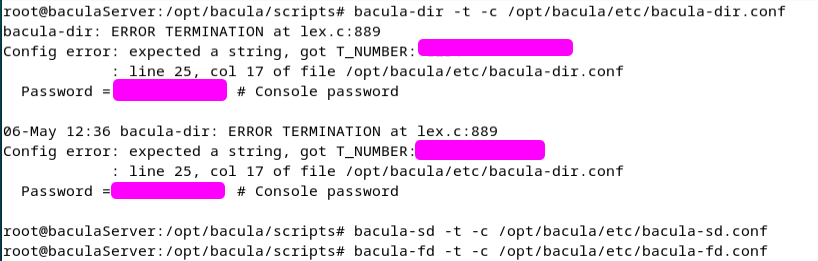
\includegraphics[width=0.5\linewidth]{instalacionBacula/verificacionSintaxsis.png}
    \caption{Ejemplo de un error de sintaxis detectado donde una contraseña es incorrectamente interpretada como un número.}
\end{figure}

Este ejemplo ilustra la importancia de asegurarse de que todos los valores en los archivos de configuración estén correctamente formateados y del tipo de dato adecuado.
